\documentclass{article}
\usepackage{amsmath,amssymb,amsfonts}
\usepackage{graphicx}
\usepackage{hyperref}
\usepackage{bookmark}
\usepackage{pgfplots}
\pgfplotsset{compat=1.18}

\title{Math Notes: 3D Graph}
\author{Trell}
\begin{document}
\maketitle


\begin{figure}[h]
    \centering
    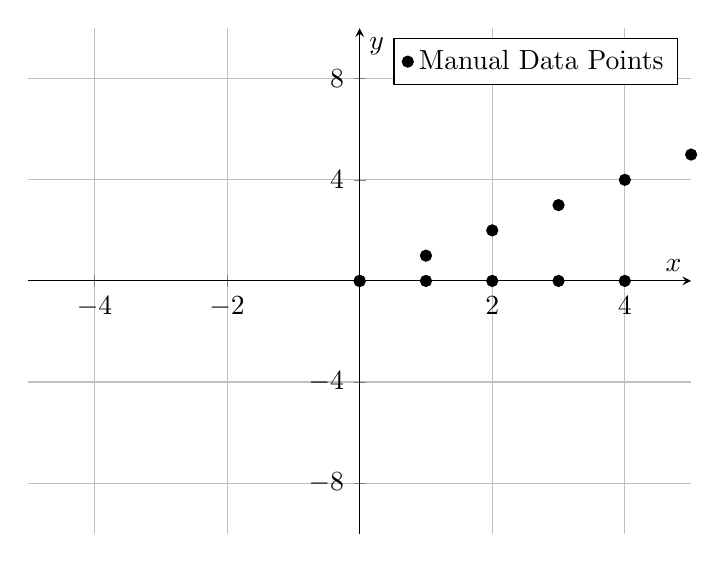
\begin{tikzpicture}
  \begin{axis}[
            axis lines = middle,
            xlabel = $x$, ylabel = $y$, 
            xmin = -5, xmax = 5,
            ymin = -10, ymax = 10,
            xtick = {-4,-2,0,2,4},
            ytick = {-8,-4,0,4,8},
            grid = major,
            width = 10cm,
            height = 8cm,
        ]
        % Manually adding points
        \addplot[only marks,mark=*] coordinates {
            (0,0)
            (1,0)
            (2,0)
            (3,0)
            (4,0)
        };

        \addplot[only marks,mark=*] coordinates {
            (0,0)
            (1,1)
            (2,2)
            (3,3)
            (4,4)
            (5,5)
        };
        
        \legend{Manual Data Points}  % Add a legend for clarity
        \end{axis}
    \end{tikzpicture}
    \caption{3D Graph of $z = \sin(x) \cdot \cos(y)$}
    \label{fig:3d-graph}


\end{figure}
\section{Trig Vocab}

\textbf{Theta}: \(\theta \) represents a angle 





\textbf{Radi}: two radi to form a sector and the arc that connects the endpoitns of the radii also has a length of r equal to the radi , the angle between the radii will be one radian 
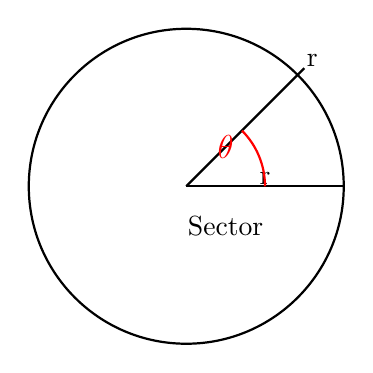
\begin{tikzpicture}
    % Draw the circle with black outline
    \draw[thick] (0,0) circle(2);

    % Draw two radii
    \draw[thick] (0,0) -- (2,0); % First radius
    \draw[thick] (0,0) -- (1.5,1.5); % Second radius

    % Label the radii with 'r'
    \node at (1,0.1) {r};
    \node at (1.6,1.6) {r};

    % Highlight the angle between the radii
    \draw[red, thick] (1,0) arc[start angle=0, end angle=45, radius=1];

    % Label the angle (between the radii)
    \node at (0.5, 0.5) {\textcolor{red}{\large $\theta$}};
    
    % Label the sector (optional)
    \node at (0.5, -0.5) {Sector};
\end{tikzpicture}
\section{Vocab And Formulas}

\textbf{Circumference} - The circumference of a circle is the total distance around the edge of the circle. It's like the perimeter of a circle.

\textbf{Radius} - The radius of a circle is the straight-line distance from the center of the circle to any point on its edge.

\textbf{Converting Degress to Radians & vice versa } -  R = (D/180)\(\pi \) , D = (R/\(\pi \))180
\section{Notes}
360 degress is one revolution and makes a circle

2 \(\pi \ ) radians = 360 degress
 \(\pi \ ) radians=  180 degress
 \(\pi \ )/2 radians=  90 degress
 \(\pi \ )/4 radians=  45 degress

 \section{Equations}

 \textbf{Finding Radius} - diamater divided by two radius = $\frac{diamater}{2}

 \section{Practice Problems}
 \textbf{Convert angles from Radians to Degrees}
 4\(\pi\)\3 = 240

 \textbf{Convert angles from Degrees to Radians}
 315 degress = 
\end{document}
